\subsection{Nearest Neighbor} \label{subsec:nearest-neighbor}

The \textbf{Nearest Neighbor Interpolation} takes an image $I_{M\times N}$ and new image dimensions $M'\times N'$ and resizes the image. Our \textit{transformed image} $I'_{M'\times N'}$ is obtained by applying the following transformation:

\[I'(x, y)=I\left(\left[\frac{x}{r_x}\right], \left[\frac{y}{r_y}\right]\right)\]

where $[x]$ denotes the nearest integer to $x$ and

\begin{align*} r_x &= \frac{M'}{M}\\
               r_y &= \frac{N'}{N}
\end{align*} are the \textit{scale factors}. In other words, we divide the values of $x$ and $y$ by their respective scale factors and look for the closest pixel in the original image, then assign the intensity value of that pixel to our transformed image. 

\begin{figure}[H]
    \centering
    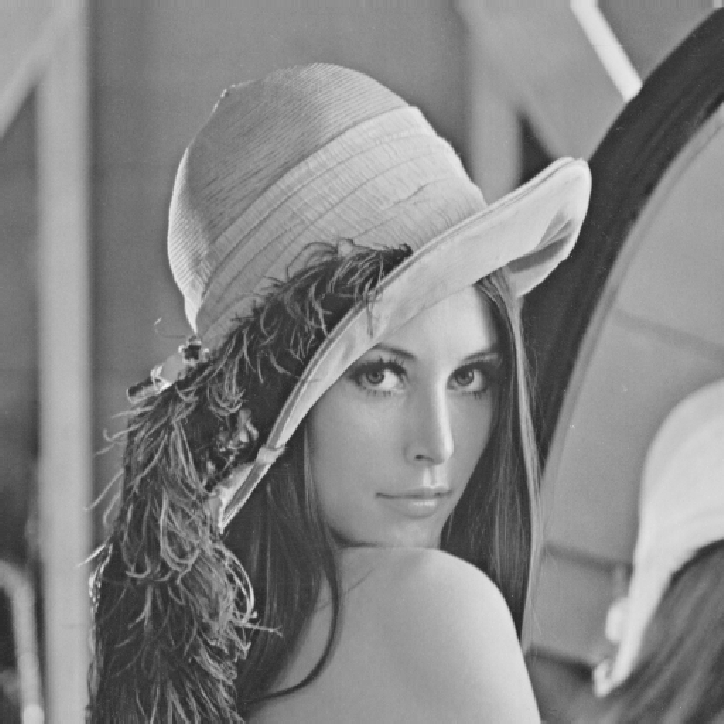
\includegraphics[scale=0.5]{images/lenna-nearest-neighbor.png}
    \caption{Nearest Neighbor Interpolation with scale $(\sqrt{2}, \sqrt{2})$}
    \label{fig:lenna-nearest-neighbor}
\end{figure}